\documentclass{standalone}
\usepackage{tikz}
\usetikzlibrary{patterns, positioning}

\begin{document}
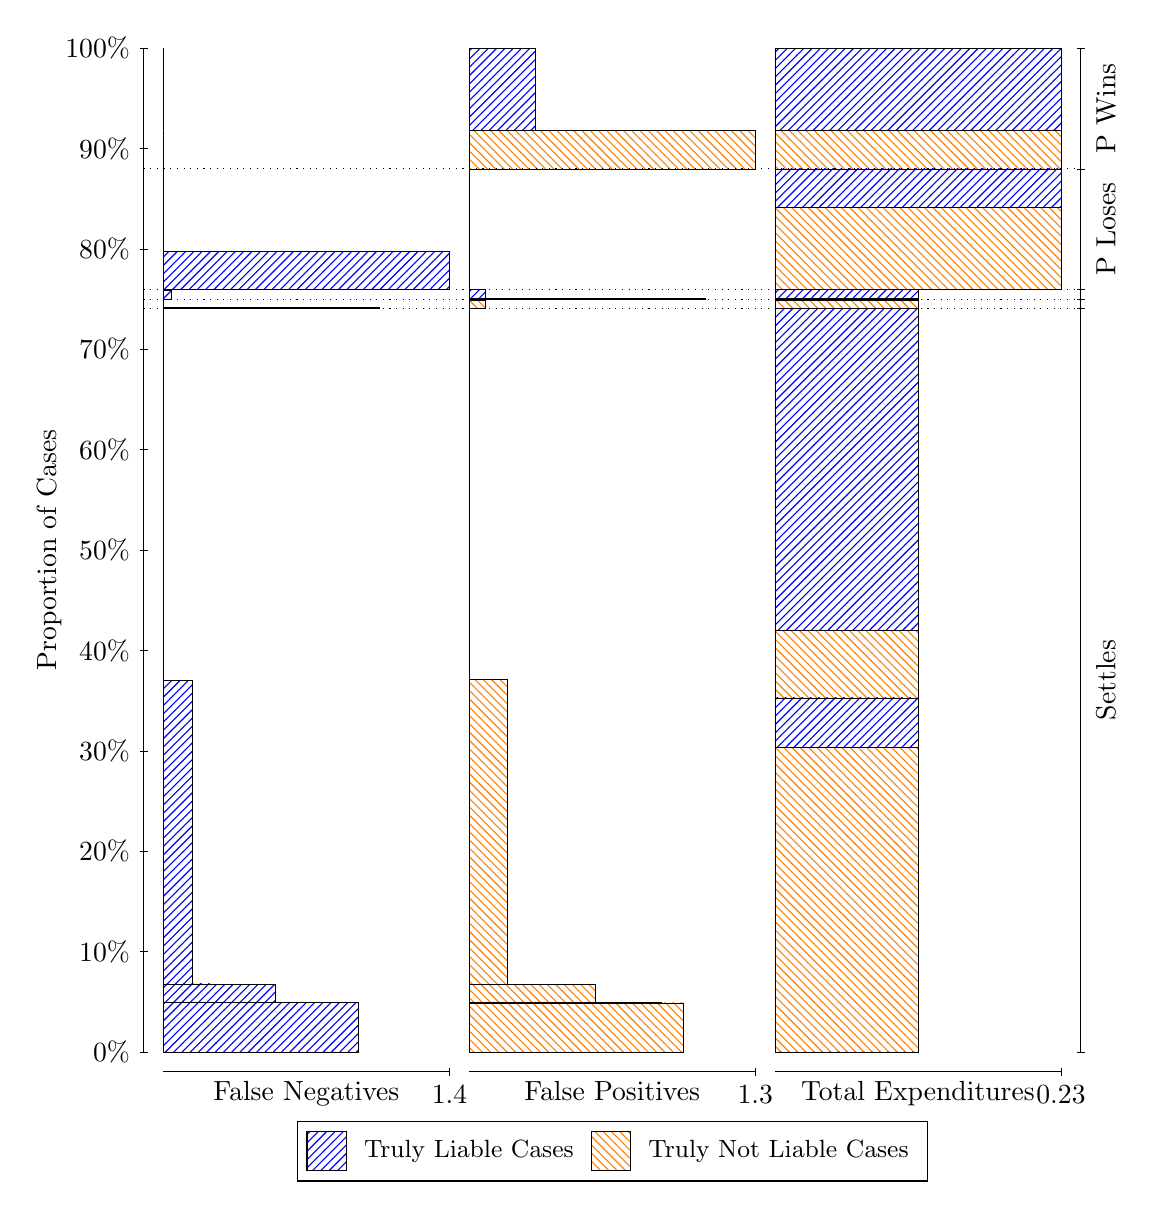
\begin{tikzpicture}
\draw[black, very thin] (1.5,1.75) -- (1.5,14.5);
\node[rotate=90, anchor=center] at (0.3, 8.125) {Proportion of Cases};
\draw[black, very thin] (1.45,1.75) -- (1.55,1.75);
\node[anchor=east] at (1.45, 1.75) {0\%};
\draw[black, very thin] (1.45,3.025) -- (1.55,3.025);
\node[anchor=east] at (1.45, 3.025) {10\%};
\draw[black, very thin] (1.45,4.3) -- (1.55,4.3);
\node[anchor=east] at (1.45, 4.3) {20\%};
\draw[black, very thin] (1.45,5.575) -- (1.55,5.575);
\node[anchor=east] at (1.45, 5.575) {30\%};
\draw[black, very thin] (1.45,6.85) -- (1.55,6.85);
\node[anchor=east] at (1.45, 6.85) {40\%};
\draw[black, very thin] (1.45,8.125) -- (1.55,8.125);
\node[anchor=east] at (1.45, 8.125) {50\%};
\draw[black, very thin] (1.45,9.4) -- (1.55,9.4);
\node[anchor=east] at (1.45, 9.4) {60\%};
\draw[black, very thin] (1.45,10.675) -- (1.55,10.675);
\node[anchor=east] at (1.45, 10.675) {70\%};
\draw[black, very thin] (1.45,11.95) -- (1.55,11.95);
\node[anchor=east] at (1.45, 11.95) {80\%};
\draw[black, very thin] (1.45,13.225) -- (1.55,13.225);
\node[anchor=east] at (1.45, 13.225) {90\%};
\draw[black, very thin] (1.45,14.5) -- (1.55,14.5);
\node[anchor=east] at (1.45, 14.5) {100\%};

\draw[black, very thin] (13.4,1.75) -- (13.4,14.5);
\draw[black, very thin] (13.35,1.75) -- (13.45,1.75);
\node[anchor=west] at (13.35, 1.75) {};
\draw[black, very thin] (13.35,11.196) -- (13.45,11.196);
\node[anchor=west] at (13.35, 11.196) {};
\draw[black, very thin] (13.35,11.308) -- (13.45,11.308);
\node[anchor=west] at (13.35, 11.308) {};
\draw[black, very thin] (13.35,11.432) -- (13.45,11.432);
\node[anchor=west] at (13.35, 11.432) {};
\draw[black, very thin] (13.35,12.966) -- (13.45,12.966);
\node[anchor=west] at (13.35, 12.966) {};
\draw[black, very thin] (13.35,14.5) -- (13.45,14.5);
\node[anchor=west] at (13.35, 14.5) {};

\draw[black, very thin, pattern color=blue, pattern=north east lines] (1.75,1.75) rectangle (4.2273,2.3757);
\draw[black, very thin, pattern color=blue, pattern=north east lines] (1.75,2.3757) rectangle (3.963,2.3767);
\draw[black, very thin, pattern color=blue, pattern=north east lines] (1.75,2.3767) rectangle (3.6988,2.3777);
\draw[black, very thin, pattern color=blue, pattern=north east lines] (1.75,2.3777) rectangle (3.4345,2.3788);
\draw[black, very thin, pattern color=blue, pattern=north east lines] (1.75,2.3788) rectangle (3.1703,2.6122);
\draw[black, very thin, pattern color=blue, pattern=north east lines] (1.75,2.6122) rectangle (2.9061,2.6126);
\draw[black, very thin, pattern color=blue, pattern=north east lines] (1.75,2.6126) rectangle (2.6418,2.613);
\draw[black, very thin, pattern color=blue, pattern=north east lines] (1.75,2.613) rectangle (2.3776,2.6135);
\draw[black, very thin, pattern color=blue, pattern=north east lines] (1.75,2.6135) rectangle (2.1133,6.4677);
\draw[black, very thin, pattern color=orange, pattern=north west lines] (1.75,6.4677) rectangle (1.75,11.196);
\draw[black, very thin, pattern color=blue, pattern=north east lines] (1.75,11.196) rectangle (4.4915,11.207);
\draw[black, very thin, pattern color=orange, pattern=north west lines] (1.75,11.207) rectangle (1.75,11.308);
\draw[black, very thin, pattern color=blue, pattern=north east lines] (1.75,11.308) rectangle (1.8491,11.42);
\draw[black, very thin, pattern color=orange, pattern=north west lines] (1.75,11.42) rectangle (1.75,11.432);
\draw[black, very thin, pattern color=blue, pattern=north east lines] (1.75,11.432) rectangle (5.3833,11.918);
\draw[black, very thin, pattern color=orange, pattern=north west lines] (1.75,11.918) rectangle (1.75,12.966);
\draw[black, very thin, pattern color=orange, pattern=north west lines] (1.75,12.966) rectangle (1.75,13.452);
\draw[black, very thin, pattern color=blue, pattern=north east lines] (1.75,13.452) rectangle (1.75,14.5);
\draw[black, very thin, pattern color=orange, pattern=north west lines] (5.6333,1.75) rectangle (8.3583,2.3745);
\draw[black, very thin, pattern color=orange, pattern=north west lines] (5.6333,2.3745) rectangle (8.0788,2.3755);
\draw[black, very thin, pattern color=orange, pattern=north west lines] (5.6333,2.3755) rectangle (7.7994,2.3763);
\draw[black, very thin, pattern color=orange, pattern=north west lines] (5.6333,2.3763) rectangle (7.5199,2.3771);
\draw[black, very thin, pattern color=orange, pattern=north west lines] (5.6333,2.3771) rectangle (7.2404,2.6107);
\draw[black, very thin, pattern color=orange, pattern=north west lines] (5.6333,2.6107) rectangle (6.9609,2.6107);
\draw[black, very thin, pattern color=orange, pattern=north west lines] (5.6333,2.6107) rectangle (6.9609,2.6113);
\draw[black, very thin, pattern color=orange, pattern=north west lines] (5.6333,2.6113) rectangle (6.6814,2.6118);
\draw[black, very thin, pattern color=orange, pattern=north west lines] (5.6333,2.6118) rectangle (6.4019,2.6123);
\draw[black, very thin, pattern color=orange, pattern=north west lines] (5.6333,2.6123) rectangle (6.1224,6.4784);
\draw[black, very thin, pattern color=blue, pattern=north east lines] (5.6333,6.4784) rectangle (5.6333,11.196);
\draw[black, very thin, pattern color=orange, pattern=north west lines] (5.6333,11.196) rectangle (5.8429,11.297);
\draw[black, very thin, pattern color=blue, pattern=north east lines] (5.6333,11.297) rectangle (5.6333,11.308);
\draw[black, very thin, pattern color=orange, pattern=north west lines] (5.6333,11.308) rectangle (8.6378,11.319);
\draw[black, very thin, pattern color=blue, pattern=north east lines] (5.6333,11.319) rectangle (5.8429,11.432);
\draw[black, very thin, pattern color=orange, pattern=north west lines] (5.6333,11.432) rectangle (5.6333,12.48);
\draw[black, very thin, pattern color=blue, pattern=north east lines] (5.6333,12.48) rectangle (5.6333,12.966);
\draw[black, very thin, pattern color=orange, pattern=north west lines] (5.6333,12.966) rectangle (9.2667,13.452);
\draw[black, very thin, pattern color=blue, pattern=north east lines] (5.6333,13.452) rectangle (6.4718,14.5);
\draw[black, very thin, pattern color=orange, pattern=north west lines] (9.5167,1.75) rectangle (11.333,1.7505);
\draw[black, very thin, pattern color=blue, pattern=north east lines] (9.5167,1.7505) rectangle (11.333,1.7515);
\draw[black, very thin, pattern color=orange, pattern=north west lines] (9.5167,1.7515) rectangle (11.333,5.6186);
\draw[black, very thin, pattern color=blue, pattern=north east lines] (9.5167,5.6186) rectangle (11.333,6.2464);
\draw[black, very thin, pattern color=orange, pattern=north west lines] (9.5167,6.2464) rectangle (11.333,7.1071);
\draw[black, very thin, pattern color=blue, pattern=north east lines] (9.5167,7.1071) rectangle (11.333,11.196);
\draw[black, very thin, pattern color=orange, pattern=north west lines] (9.5167,11.196) rectangle (11.333,11.297);
\draw[black, very thin, pattern color=blue, pattern=north east lines] (9.5167,11.297) rectangle (11.333,11.308);
\draw[black, very thin, pattern color=orange, pattern=north west lines] (9.5167,11.308) rectangle (11.333,11.319);
\draw[black, very thin, pattern color=blue, pattern=north east lines] (9.5167,11.319) rectangle (11.333,11.432);
\draw[black, very thin, pattern color=orange, pattern=north west lines] (9.5167,11.432) rectangle (13.15,12.48);
\draw[black, very thin, pattern color=blue, pattern=north east lines] (9.5167,12.48) rectangle (13.15,12.966);
\draw[black, very thin, pattern color=orange, pattern=north west lines] (9.5167,12.966) rectangle (13.15,13.452);
\draw[black, very thin, pattern color=blue, pattern=north east lines] (9.5167,13.452) rectangle (13.15,14.5);
\draw[black, dotted] (1.5,11.196) -- (13.4,11.196);
\draw[black, dotted] (1.5,11.308) -- (13.4,11.308);
\draw[black, dotted] (1.5,11.432) -- (13.4,11.432);
\draw[black, dotted] (1.5,12.966) -- (13.4,12.966);
\draw[black, very thin] (1.75,1.5) -- (5.3833,1.5);
\node[anchor=north] at (3.5667, 1.5) {False Negatives};
\draw[black, very thin] (5.3833,1.45) -- (5.3833,1.55);
\node[anchor=north] at (5.3833, 1.45) {1.4};

\draw[black, very thin] (5.6333,1.5) -- (9.2667,1.5);
\node[anchor=north] at (7.45, 1.5) {False Positives};
\draw[black, very thin] (9.2667,1.45) -- (9.2667,1.55);
\node[anchor=north] at (9.2667, 1.45) {1.3};

\draw[black, very thin] (9.5167,1.5) -- (13.15,1.5);
\node[anchor=north] at (11.333, 1.5) {Total Expenditures};
\draw[black, very thin] (13.15,1.45) -- (13.15,1.55);
\node[anchor=north] at (13.15, 1.45) {0.23};

\node[black, centered, rotate=90] at (13.72, 6.473) {Settles};


\node[black, centered, rotate=90] at (13.72, 12.199) {P Loses};
\node[black, centered, rotate=90] at (13.72, 13.733) {P Wins};

\draw (7.449999999999999,1.5) node[draw=none] (baseCoordinate) {};
\begin{scope}[align=center]
        \matrix[scale=0.5, draw=black, below=0.5cm of baseCoordinate, nodes={draw}, column sep=0.1cm]{
            \node[rectangle, draw, minimum width=0.5cm, minimum height=0.5cm, pattern=north east lines, pattern color=blue] {}; &
            \node[draw=none, font=\small] (B) {Truly Liable Cases}; &
            \node[rectangle, draw, minimum width=0.5cm, minimum height=0.5cm, pattern=north west lines, pattern color=orange] {}; &
            \node[draw=none, font=\small] (B) {Truly Not Liable Cases}; \\
            };
\end{scope}

\end{tikzpicture}
\end{document}